\documentclass[11pt]{article}
\usepackage{amsmath, amssymb}
\usepackage{geometry}
\geometry{margin=1in}
\usepackage{fancyhdr}
\usepackage{lastpage}
\usepackage{parskip} % Better paragraph spacing
\usepackage{titlesec} % Better section formatting
\usepackage{graphicx}
\usepackage{float}
\usepackage[most]{tcolorbox}
\usepackage{lmodern}
\usepackage{caption}

% Define commands for reusable content
\newcommand{\coursename}{COM-407 Advanced Networks}
\newcommand{\lecturenum}{05}
\newcommand{\lecturedate}{\today}
\newcommand{\professor}{Pavlos Nikolopoulos}

% Configure section spacing
\titlespacing*{\section}{0pt}{2ex plus 1ex minus .2ex}{1.5ex plus .2ex}
% Header / Footer
\pagestyle{fancy}
\fancyhf{}
\fancyhead[L]{\coursename}
\fancyhead[R]{Lecture \lecturenum}
\fancyfoot[L]{EPFL - Computer Science}
\fancyfoot[C]{Author: Jonathan Dutoit}
\fancyfoot[R]{Page \thepage\ of \pageref{LastPage}}

\begin{document}

\begin{center}
  {\large EPFL - Computer Science} \\[0.5em]
  {\Large \textbf{\coursename}} \\[0.5em]
  {\large Lecture \lecturenum\ --- \lecturedate} \\[0.5em]
  {\large Author: Jonathan Dutoit} \\[0.5em]
  {\large Professor: \professor} \\[0.5em]
\end{center}

\vspace{2cm}
\begin{center}
  {\LARGE \textbf{MAC Layer (continued)}}
\end{center}

\vspace{1cm}
\section*{2. (Today's) Switched Ethernet}

Today, Ethernet is based on: 
\begin{itemize}
	\item \textcolor{red}{switches} (or \textcolor{red}{bridges}):
		\begin{itemize}
			\item middle boxes of the MAC layer
			\item queing systems (with frame buffers) that forward frames based on MAC addresses
		\end{itemize}
	\item \textcolor{blue}{full-duplex cables}:
		\begin{itemize}
			\item frames flow simultaneously in both directions without suffering collisions (\textcolor{blue}{collision-less} ethernet) 
			\item e.g., the well-known UTP cables with separate downlink/uplink
		\end{itemize}
\end{itemize}

% Quick centered image
\begin{figure}[H]
    \centering
    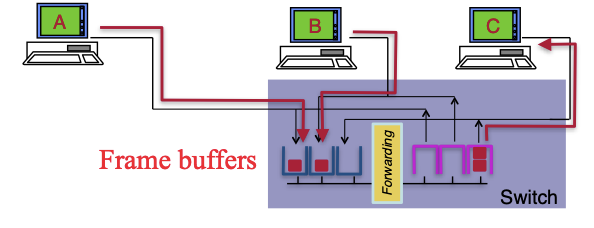
\includegraphics[width=0.7\textwidth]{images/switches}
    \label{fig:LABEL}
\end{figure}

\textbf{Is switched Ethernet a different protocol?}

No, switches are designed to be \textcolor{red}{transparent}:

i.e. there should be \textcolor{blue}{no difference} for the protocol used by end-system when they are connected to a coax cable, concentrator/hub or a switch/bridge 

But, since we can't get collisions, \textcolor{blue}{CSMA/CD is disabled} by default.

% Quick centered image
\begin{figure}[H]
    \centering
    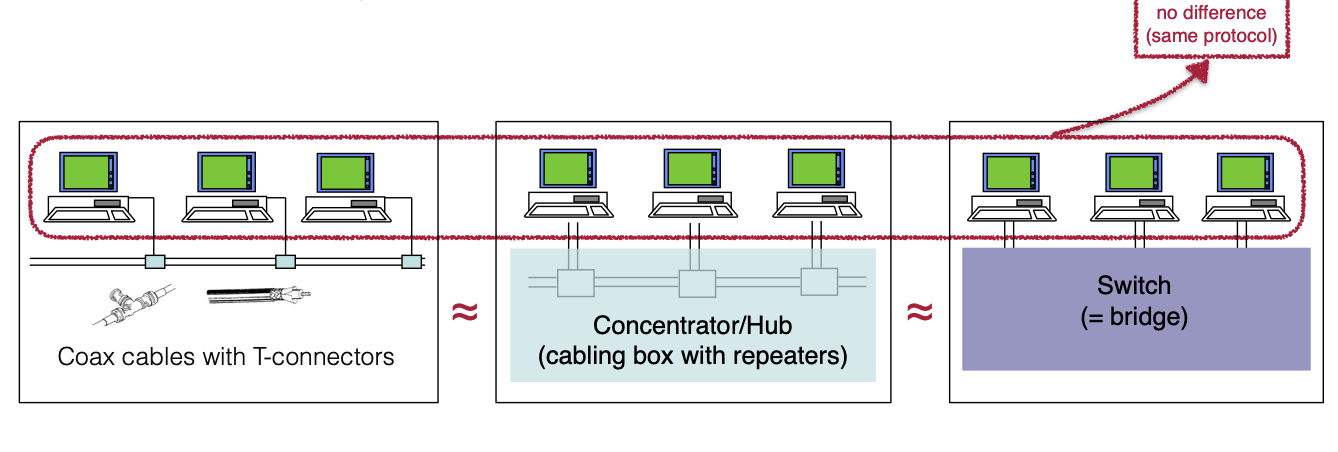
\includegraphics[width=0.8\textwidth]{images/same-protocol}
    \label{fig:LABEL}
\end{figure}

\begin{tcolorbox}[
  colback=gray!15,     % background color
  colframe=black!50,    % border color
  boxrule=1pt,       % border thickness
  arc=3mm,             % rounded corners
  left=4mm, right=4mm, top=2mm, bottom=2mm % padding
]
\textbf{How many frames can be transmitted in parallel in this switched Ethernet LAN (all boxes are switches)?}
% Quick centered image
\begin{figure}[H]
    \centering
    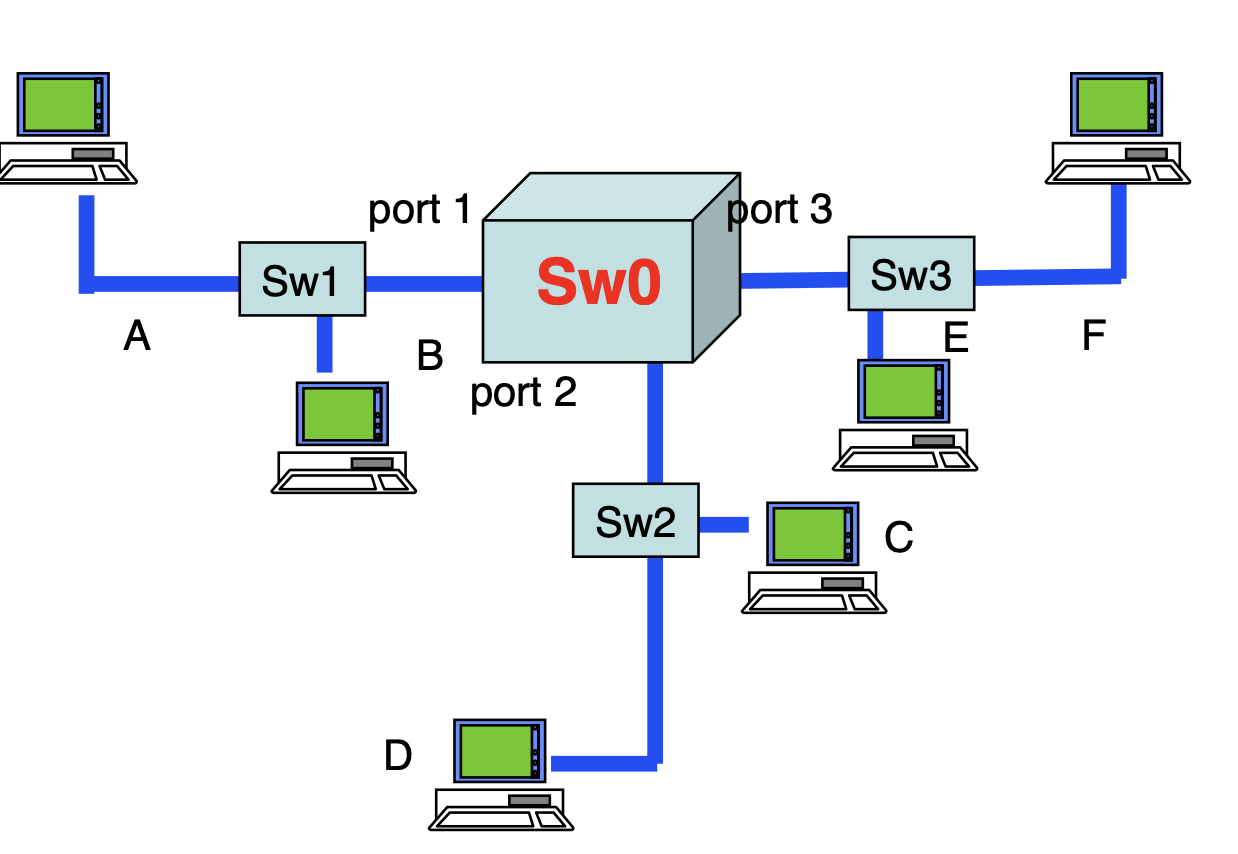
\includegraphics[width=0.5\textwidth]{images/switches-question}
    \label{fig:LABEL}
\end{figure}
\vspace{0.3cm}

A. 1 \\
B. 3 \\
C. 6 \\
D. $>$ 6 \\
E. I don't know \\

 \textbf{Answer:} D \\

 Assume that switches can transmit on all ports in parallel (one LAN adapter per port). \\

 Since switches are \textcolor{red}{full duplex}, there can be up to 2 frames transmissions on every link (one in each direction), therefore up to 18 transmissions in parallel \\

 $\Rightarrow$  \textcolor{blue}{this is the benefit of today's switches over shared-medium, old-style Ethernet}
\end{tcolorbox}

\section*{How does a switch forward a frame?}

\begin{itemize}
	\item Switches use:
		\begin{itemize}
			\item a forwarding table with \textcolor{red}{exact match} \\
		which maps destination MAC addresses to outgoing interfaces (a.k.a. "ports")
			\item and a \textcolor{blue}{forwarding algorithm}	
		\end{itemize}
	\item Smart switches handle \textcolor{blue}{multicast frames differently}
\end{itemize}

% Quick centered image
\begin{figure}[H]
    \centering
    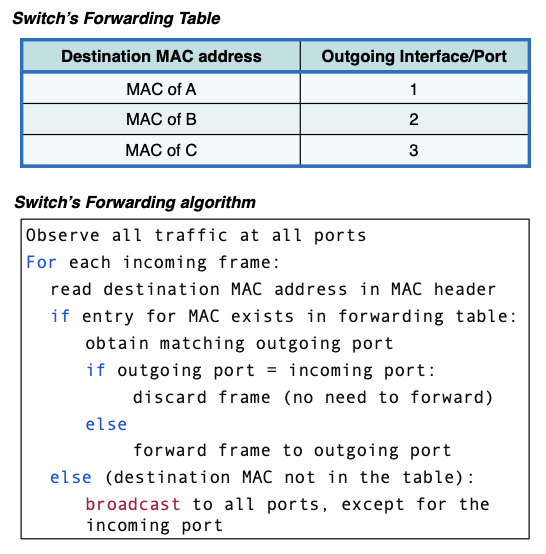
\includegraphics[width=0.7\textwidth]{images/forwarding-algo}
    \label{fig:LABEL}
\end{figure}

\section*{How does a switch populate its forwarding table?}

By observing traffic (\textcolor{red}{plug-and-play device}):
\begin{itemize}
	\item table build by \textcolor{blue}{self-learning} from source MAC address field in incoming frames
	\item learnt addresses time out if not re-learnt after an \textcolor{blue}{ageing time}
\end{itemize}

$\Rightarrow$  \textcolor{red}{different} from IP routers that use routing algorithms

\begin{tcolorbox}[
  colback=gray!15,     % background color
  colframe=black!50,    % border color
  boxrule=1pt,       % border thickness
  arc=3mm,             % rounded corners
  left=4mm, right=4mm, top=2mm, bottom=2mm % padding
]
\textbf{Can self learning be extended to inter-connected switches?}

\vspace{0.3cm}

A. Yes because learning propagates \\
B. Yes because MAC addresses are unstructured \\
C. Only in some special cases \\
D. No, never \\
E. I don't know \\

\textbf{Answer:} C \\

It does not work if there are \textcolor{red}{loops} in the topology

% Quick centered image
\begin{figure}[H]
    \centering
    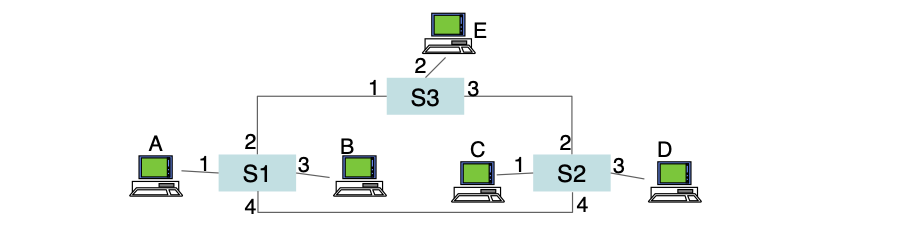
\includegraphics[width=0.7\textwidth]{images/learning-connection}
    \label{fig:LABEL}
\end{figure}

E.g.: here S3 does not know whether A is on port 1 or 3, as flooded/broadcast packets may arrive from either side. (Recall that switches are queueing systems, hence there exist non-deterministic delays) \\

$\Rightarrow$ The entries of the forwarding table may change  \textcolor{red}{indefinitely} and packets may be trapped in a link, as we saw when talking about TTL in IP layer.
\end{tcolorbox}

\section*{Spanning Tree Protocol (STP): the common way to prevent loops}

\begin{minipage}{0.5\textwidth}
\textcolor{red}{What does it do?} \\

\begin{itemize}
	\item forces the active topology to be a \textcolor{blue}{tree} (i.e. loop-free) that spans all switches by \textcolor{blue}{deactivating} some links 
	\item adapts to link failures and additions whenever needed
\end{itemize}

\end{minipage}
\hfill
\begin{minipage}{0.5\textwidth}
\centering
\includegraphics[width=\linewidth]{stp}
\end{minipage}

\section*{How does the Spanning Tree Protocol work?}

The switches: 

1. elect a \textcolor{red}{root} switch = switch with smallest (configurable) label ID

2. activate only the links that are along the shortest path to root switch. The spanning tree = set of \textcolor{blue}{shortest paths} to root switch

3. monitor whether the root is reachable, and if not, they trigger a re-computation of a new spanning tree

% Quick centered image
\begin{figure}[H]
    \centering
    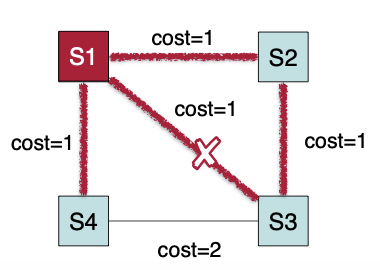
\includegraphics[width=0.5\textwidth]{images/stp-2}
    \label{fig:LABEL}
\end{figure}

\textbf{a few important points}: 

\begin{itemize}
	\item STP is a \textcolor{red}{distributed} algorithm
		\begin{itemize}
			\item no central control
			\item everything is \textcolor{blue}{plug and play}
			\item a \textcolor{blue}{gossip} protocol is used to learn the IDs
		\end{itemize}
	\item Shortest paths = paths incurring the smallest aggregate cost to the root
		\begin{itemize}
			\item each link between switches has a (configurable) \textcolor{red}{cost}
			\item typically, the cost is a decreasing function of bit rate
		\end{itemize}
	\item Switches compute the shortest paths using a variant of \textcolor{blue}{Bellman-Ford} algorithm
\end{itemize}

\begin{tcolorbox}[
  colback=gray!15,     % background color
  colframe=black!50,    % border color
  boxrule=1pt,       % border thickness
  arc=3mm,             % rounded corners
  left=4mm, right=4mm, top=2mm, bottom=2mm % padding
]
\textbf{Which of the following links are on the spanning tree ?}
% Quick centered image
\begin{figure}[H]
    \centering
    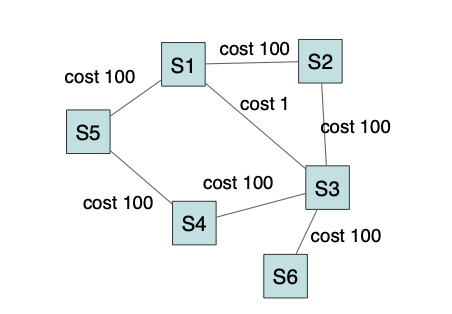
\includegraphics[width=0.5\textwidth]{images/spanning-tree-question}
    \label{fig:LABEL}
\end{figure}
\vspace{0.3cm}

A. S4-S5 \\
B. S4-S3 \\
C. Both \\
D. None \\
E. I don't know \\

\textbf{Answer:} B
\end{tcolorbox}

\section*{A side-effect of the Spanning Tree Protocol (STP)}

\begin{minipage}{0.5\textwidth}
\begin{itemize}
	\item All frames go through the spanning tree
	\item A direct link between two (non-root) switches may be not used even if its optimal 
		\begin{itemize}
			\item e.g., the path from A to B, here, is not optimal 
		\end{itemize}
	\item \textcolor{red}{Less efficient} than shortest path
	\item Some more sophisticated switches implement Shortest Path Bridging instead of STP, which is the default
\end{itemize}

\end{minipage}
\hfill
\begin{minipage}{0.5\textwidth}
\centering
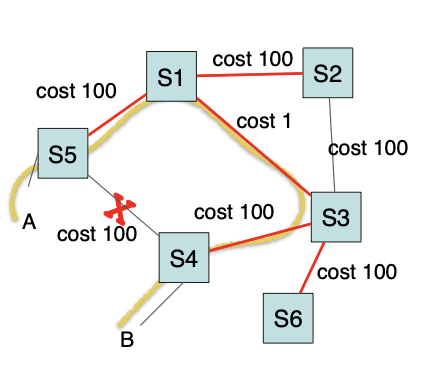
\includegraphics[width=\linewidth]{images/stp-3}
\end{minipage}

\section*{3. Ethernet Frame format}

\begin{itemize}
	\item Ethernet frame = Ethernet's Protocol Data Unit (PDU)
	\item An Ethernet frame typically carries an IP packet in its payload, sometimes also other: 
		\begin{itemize}
			\item IPv4
			\item ARP
			\item MACSEC (authenticated/encrypted frame)
			\item Precision Time Protocol
		\end{itemize}
\end{itemize}
% Quick centered image
\begin{figure}[H]
    \centering
    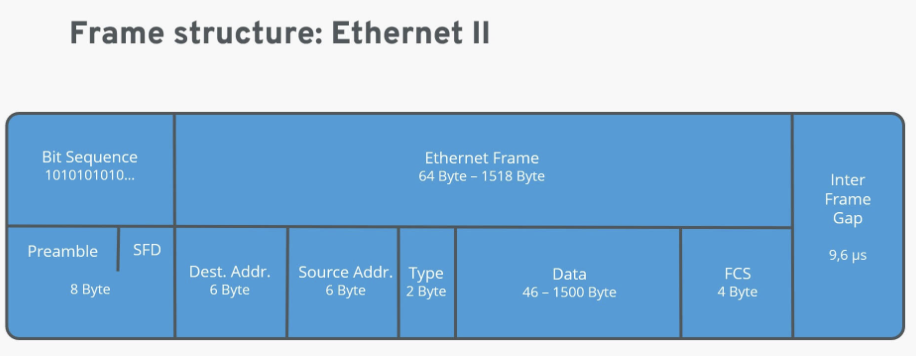
\includegraphics[width=0.9\textwidth]{images/frame2}
    \label{fig:LABEL}
\end{figure}

\textbf{preamble}: bits used to detect start of frame necessary to synchronize clocks (e.g., from receiver) which is also called delimiter. It is a bit sequences of 7 bytes, where each byte is equal to: 10101010... and it is terminated by 0.
Following the preamble, an additional byte is used to indicate the beginning of the frame. This is called SFD (=start frame delimiter) and its similar to a preamble byte, but its last two bits are 11 (instead of 10).

In Ethernet, transmission starts \textcolor{blue}{asynchronously} (host transmit independently), and between transmissions, the channel is idle. This is why the clocks of the send and the receiver have to get synchronized at the beginning of each frame. 

There is no frame length field in the Ethernet header -- its up to the higher layer using Ethernet to find out the length of the payload. 

Frames have to be at least 64B (to see why, refer to minimum frame size) and at most 1500B. If needed, padding is inserted to make the frame long enough, and only in that case the Type field is used to indicate the length of the size of the payload before padding. 

\section*{Error Detection via Frame Check Sequence (FCS)}
\textcolor{red}{Why?}

\begin{itemize}
	\item The channel may cause bit errors during transmission $\Rightarrow$ a frame may be "\textcolor{red}{corrupted}"
	\item We want to detect and discard corrupted frames.
\end{itemize}
\textcolor{red}{How?}
\begin{itemize}
	\item The sender computes a Cyclic Redundancy Checksum (CRC, 32bits) of the frame and inserts it in the FCS field
	\item The receiver recomputes the CRC checksum and checks if it is equal to the FCS
	\item CRC can \textcolor{blue}{detect} all single, double, triple errors, all error bursts of length $\leq$ 32, most double burst of length  $\leq$ 17
		 \begin{itemize}
			\item The probability that a random collection of bit errors goes undetected is $\approx 2e-32$
		\end{itemize}
\end{itemize}

* \textcolor{red}{Error recovery} in Ethernet is simple: If a frame fails the check, it is \textcolor{red}{dropped}
\section*{MAC Unicast}

\begin{itemize}
	\item MAC address: 48 bits = adapted ID, unique worldwide (in principle, but can be also configured sometimes)
\end{itemize}

\textcolor{red}{How?}
\begin{itemize}
	\item Sender puts destination MAC address in the frame
	\item Address sent in the cleartext, no encryption
\end{itemize}

\begin{itemize}
	\item In \textcolor{red}{shared-medium} LAN: \\
	all stations read \textcolor{red}{all} frames, but keep only if the destination address matches
	\item In \textcolor{blue}{switched Ethernet}: \\
		switches forward frames \textcolor{blue}{only} to ports that need it (in principle, works differently if there's no entry in the forwarding table...)
\end{itemize}

% Quick centered image
\begin{figure}[H]
    \centering
    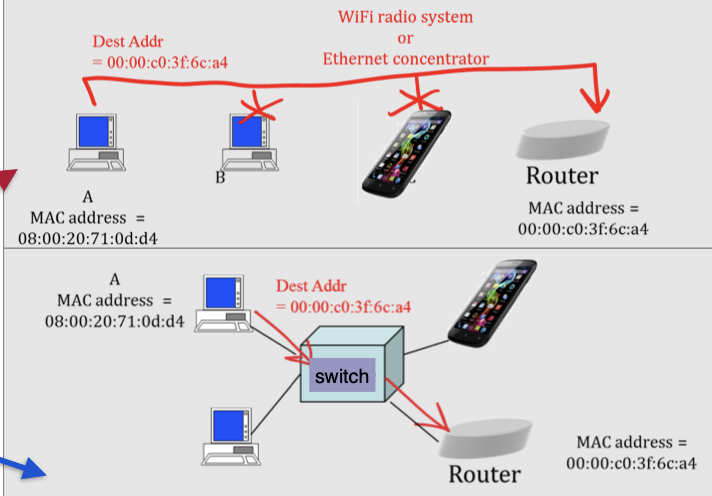
\includegraphics[width=0.8\textwidth]{images/mac-unicast}
    \label{fig:LABEL}
\end{figure}

\section*{Addressing: more details (for the interested students)}

Ethernet addresses are known as MAC addresses. Every Ethernet interface has its own MAC address, which is in fact similar to the serial number of the adapter, set by the manufacturer. 

When A sends a data frame to B, A creates a MAC frame with source addr = A, dest addr = B. The frame is sent on the network and recognized by the destination. 

The data is transmitted in Ethernet, with the least significant bit of first octet first -- this is a strange behavior dictated by Intel processors. Canonical representation thus inverts the order of bits inside a byte (the first bit of the address is the least significant bit of the first byte)

\section*{MAC Broadcast}
\begin{itemize}
	\item ff:ff:ff:ff:ff = broadcast address
	\item In \textcolor{red}{shared-medium} LAN: all machines receive packet and do \textcolor{red}{not} discard it
	\begin{center}
		% Quick centered image
		\begin{figure}[H]
		    \centering
		    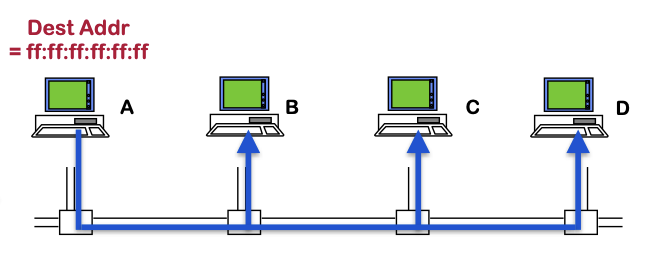
\includegraphics[width=0.5\textwidth]{images/broadcast-1}
		    \label{fig:LABEL}
		\end{figure}
	\end{center}
	\item In \textcolor{blue}{switched Ethernet}: broadcast frames are sent on all nodes and ports \textcolor{blue}{on the spanning tree}
		\begin{center}
			% Quick centered image
			\begin{figure}[H]
			    \centering
			    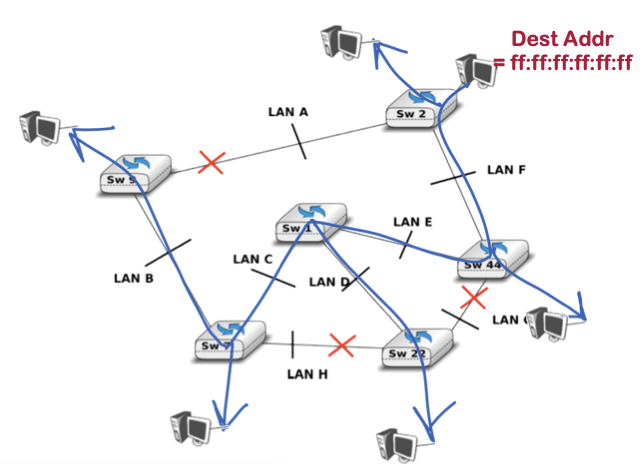
\includegraphics[width=0.5\textwidth]{images/broadcast-2}
			    \label{fig:LABEL}
			\end{figure}
		\end{center}
\end{itemize}

\section*{MAC Multicast (= sending to multiple host)}

\begin{itemize}
	\item uses:
		\begin{itemize}
			\item MAC addresses with 8th bit == 1 are multicast addresses
			\item various multicast addresses to support various protocols (e.g., IPv4, IPv6, PTP)

			% Quick centered image
			\begin{figure}[H]
			    \centering
			    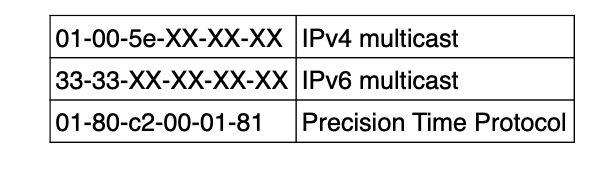
\includegraphics[width=0.5\textwidth]{images/multicast-1}
			    \label{fig:LABEL}
			\end{figure}
		\end{itemize}
	\item makes sense only in \textcolor{blue}{switched Ethernet}:
		\begin{itemize}
			\item Ethernet adapter discards multicast packets, unless host subscribes to addresses
			\item non-smart switches \textcolor{red}{broadcast} such frames
			\item smart switches send \textcolor{red}{only to relevant} hosts (the subscribed ones to the multicast group -- see "multicast" lecture)
			% Quick centered image
			\begin{figure}[H]
			    \centering
			    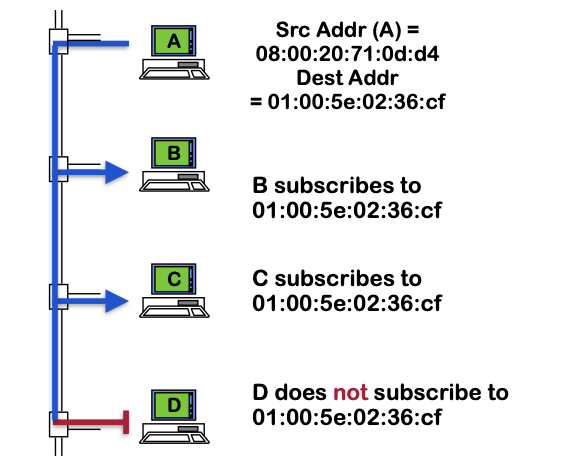
\includegraphics[width=0.5\textwidth]{images/multicast-2}
			    \label{fig:LABEL}
			\end{figure}
		\end{itemize}
\end{itemize}

\begin{tcolorbox}[
  colback=gray!15,     % background color
  colframe=black!50,    % border color
  boxrule=1pt,       % border thickness
  arc=3mm,             % rounded corners
  left=4mm, right=4mm, top=2mm, bottom=2mm % padding
]
\textbf{The protocol type in an Ethernet frame header indicates whether...}

\vspace{0.3cm}

A. ...the data is a TCP packet or not \\
B. ...the data is an IPv4 packet or not \\
C. Both \\
D. None \\
E. I don't know \\

\textbf{Answer}: B  \\

The Ethertype indicates an IPv4 or IPv6 packet
\end{tcolorbox}


\begin{tcolorbox}[
  colback=gray!15,     % background color
  colframe=black!50,    % border color
  boxrule=1pt,       % border thickness
  arc=3mm,             % rounded corners
  left=4mm, right=4mm, top=2mm, bottom=2mm % padding
]
\textbf{We have a working environment with IPv4, using Ethernet
switches plus other things. We add IPv6 to the network. Do we
need to change the switch configurations?}

\vspace{0.3cm}

A. No, since switches look only at MAC addresses. \\
B. Yes since the protocol type is different. \\
C. It depends whether SLAAC is used \\
D. I don't know  \\

\textbf{Answer}:A \\

The switches work only at MAC layer and continue to work the same whether IPv4, IPv6 (or something else) is used. \\

One \textcolor{red}{exception}: "smart" switches are cheating -- they build multicast trees by looking at IP layer group membership (see multicast lecture later)
\end{tcolorbox}

\section*{4. Virtual LANs}

\textcolor{red}{Why invented?}
\begin{itemize}
	\item Lack of traffic isolation $\rightarrow$ we want to limit the scope of broadcast traffic and have access control
	\item Inefficient use of switches $\rightarrow$ we do not want to buy extra switches if other have available ports
	\item Managing users $\rightarrow$ if a user moves, we do not want to also change its physical cabling
\end{itemize}
\textcolor{red}{\textit{Goal:}} Decouple who belongs to which LAN from their physical location

% Quick centered image
\begin{figure}[H]
    \centering
    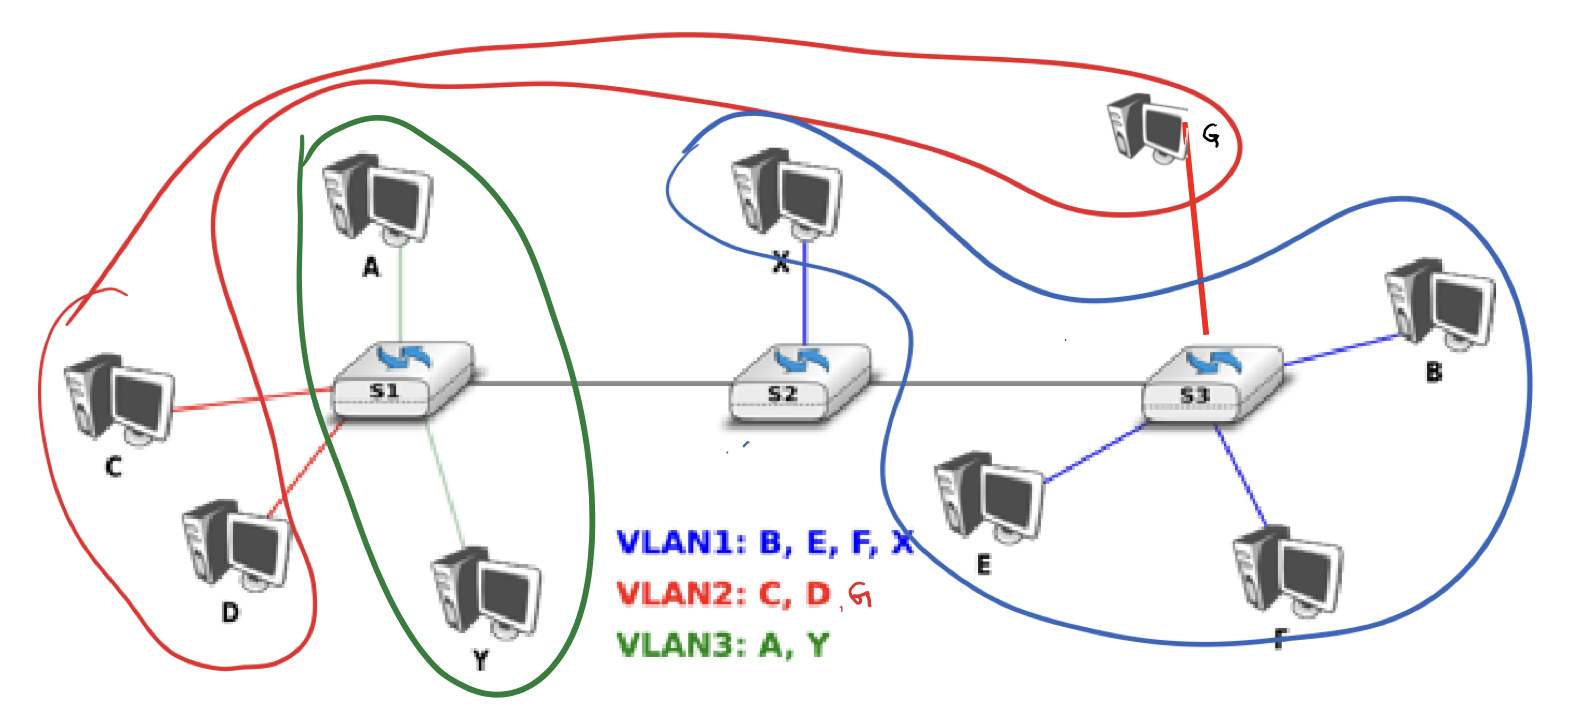
\includegraphics[width=0.8\textwidth]{images/vlan}
    \label{fig:LABEL}
\end{figure}

\begin{itemize}
	\item VLANs operate as if they were physically separate:
		\begin{itemize}
			\item different forwarding tables, different spanning trees
		\end{itemize}
	\item \textcolor{red}{\textit{How}} does it work?
		\begin{itemize}
			\item network manager configures which switch port belongs to which VLAN
			\item switch treats ports of different VLANs as separate, non communicating LANs
			\item If more than one switches implement the same VLANs, they are interconnected via \textcolor{blue}{\textit{trunk}} ports, which use VLAN tags in an Ethernet's \textcolor{blue}{\textit{extender header}}, in order to correctly associate frames with VLANs. 
		\end{itemize}
\end{itemize}

\textbf{Example of a trunk port}

% Quick centered image
\begin{figure}[H]
    \centering
    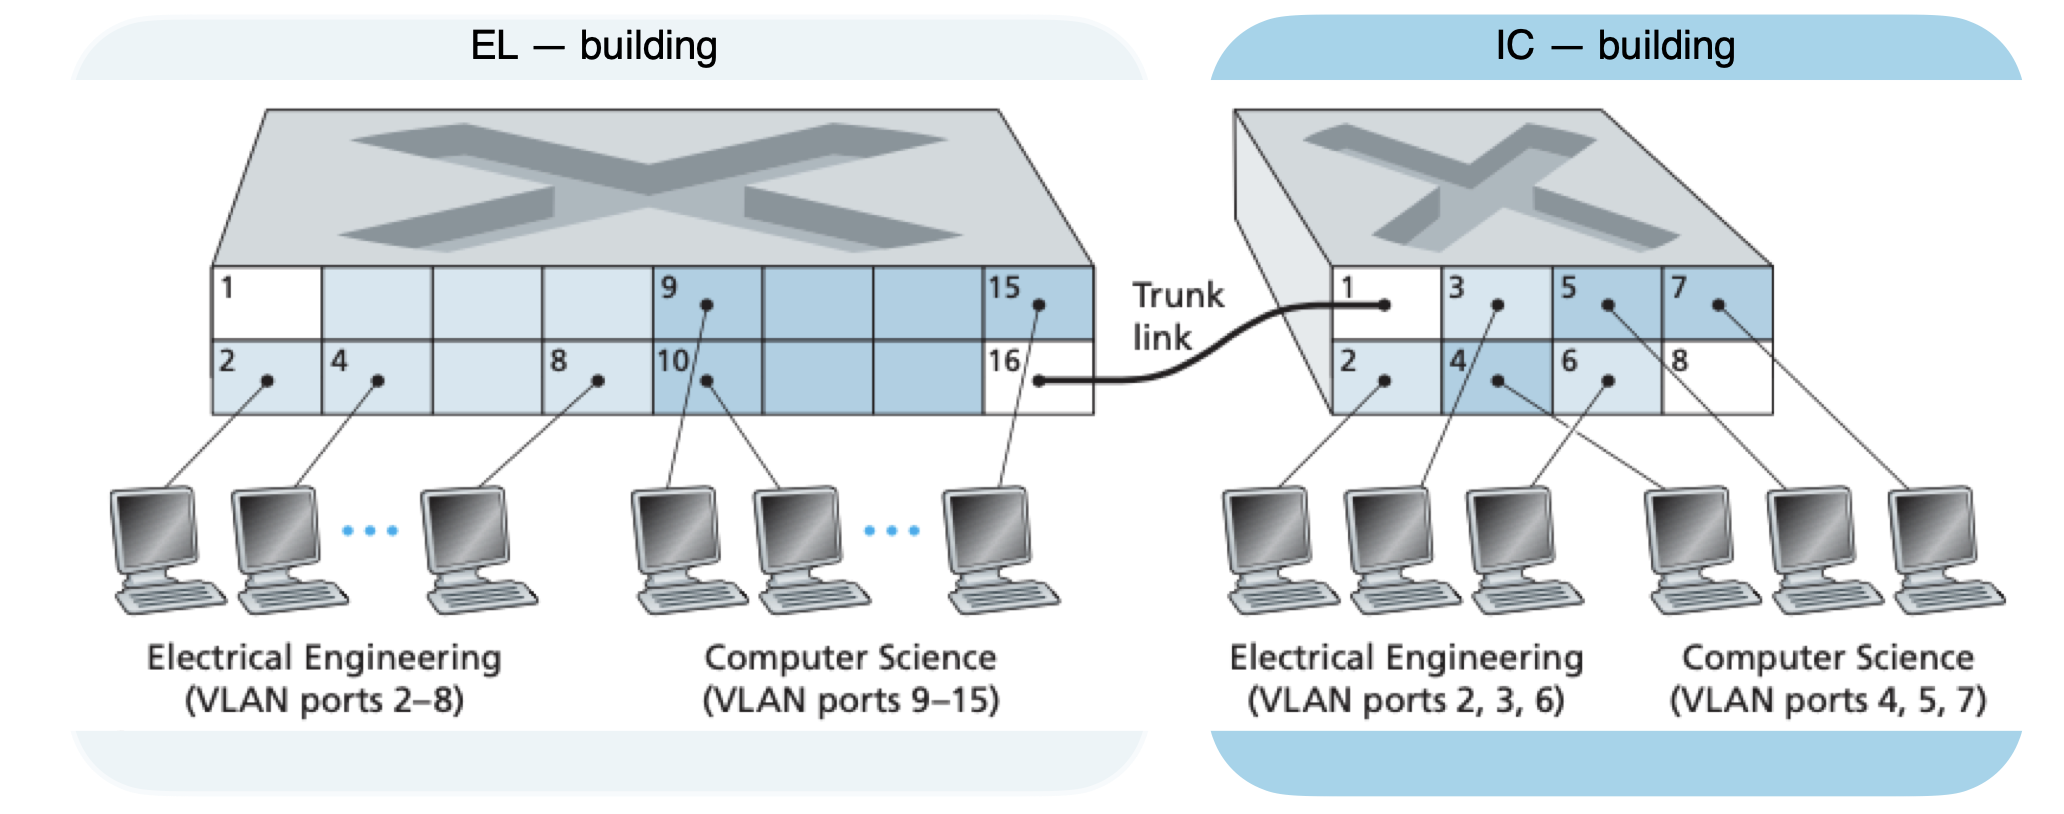
\includegraphics[width=0.8\textwidth]{images/trunk-port}
    \label{fig:LABEL}
\end{figure}

\begin{itemize}
	\item The switches implement 2 virtual LANs
		\begin{itemize}
			\item the Electrical Engineering LAN in light blue and
			\item the Computer Science LAN in a blue color
		\end{itemize}
	\item The switches are interconnected via trunk ports (16 and 1) that belong to both LANS
	\item The trunk ports use VLAN tags to notify each other which arriving frame belongs to which VLAN
\end{itemize}

\begin{tcolorbox}[
  colback=gray!15,     % background color
  colframe=black!50,    % border color
  boxrule=1pt,       % border thickness
  arc=3mm,             % rounded corners
  left=4mm, right=4mm, top=2mm, bottom=2mm % padding
]
\textbf{A has an IP packet destined to C; S1 is a switch; what should A do?}
% Quick centered image
\begin{figure}[H]
    \centering
    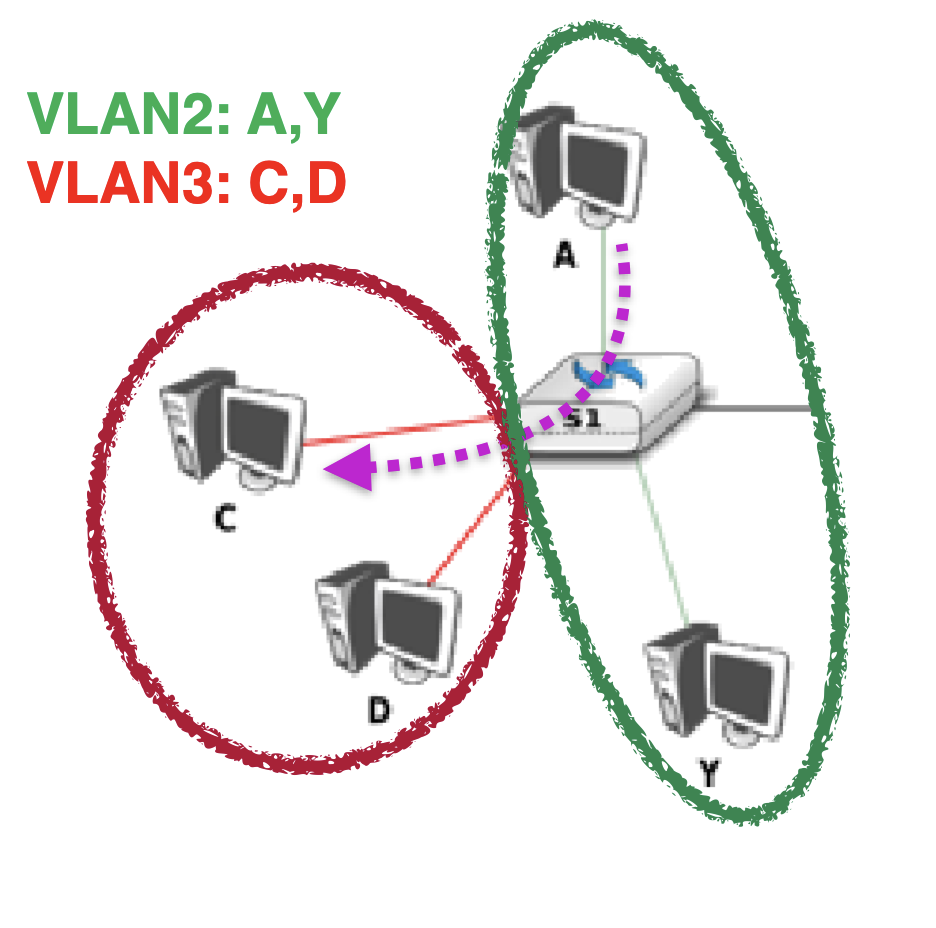
\includegraphics[width=0.3\textwidth]{images/vlan-question}
    \label{fig:LABEL}
\end{figure}
\vspace{0.3cm}
A. Send an ARP request in order to obtain the MAC address of C, then send the packet to that MAC address. \\
B. Send an ARP request in order to obtain both the MAC address and the VLAN label of C, then send the packet to this MAC address and to this VLAN \\
C. None of the above \\
D. I don't know \\

\textbf{Answer}: C. VLANs 2 and 3 are two \textit{\textcolor{red}{separate}} LANs, it is not possible for A to send directly to C - it must go through a router. 
\end{tcolorbox}


\section*{5. Bridges}

\textit{\textcolor{blue}{layer-2 devices}} that interconnected different medium-access technologies (e.g., WiFi with Ethernet) without routers

% Quick centered image
\begin{figure}[H]
    \centering
    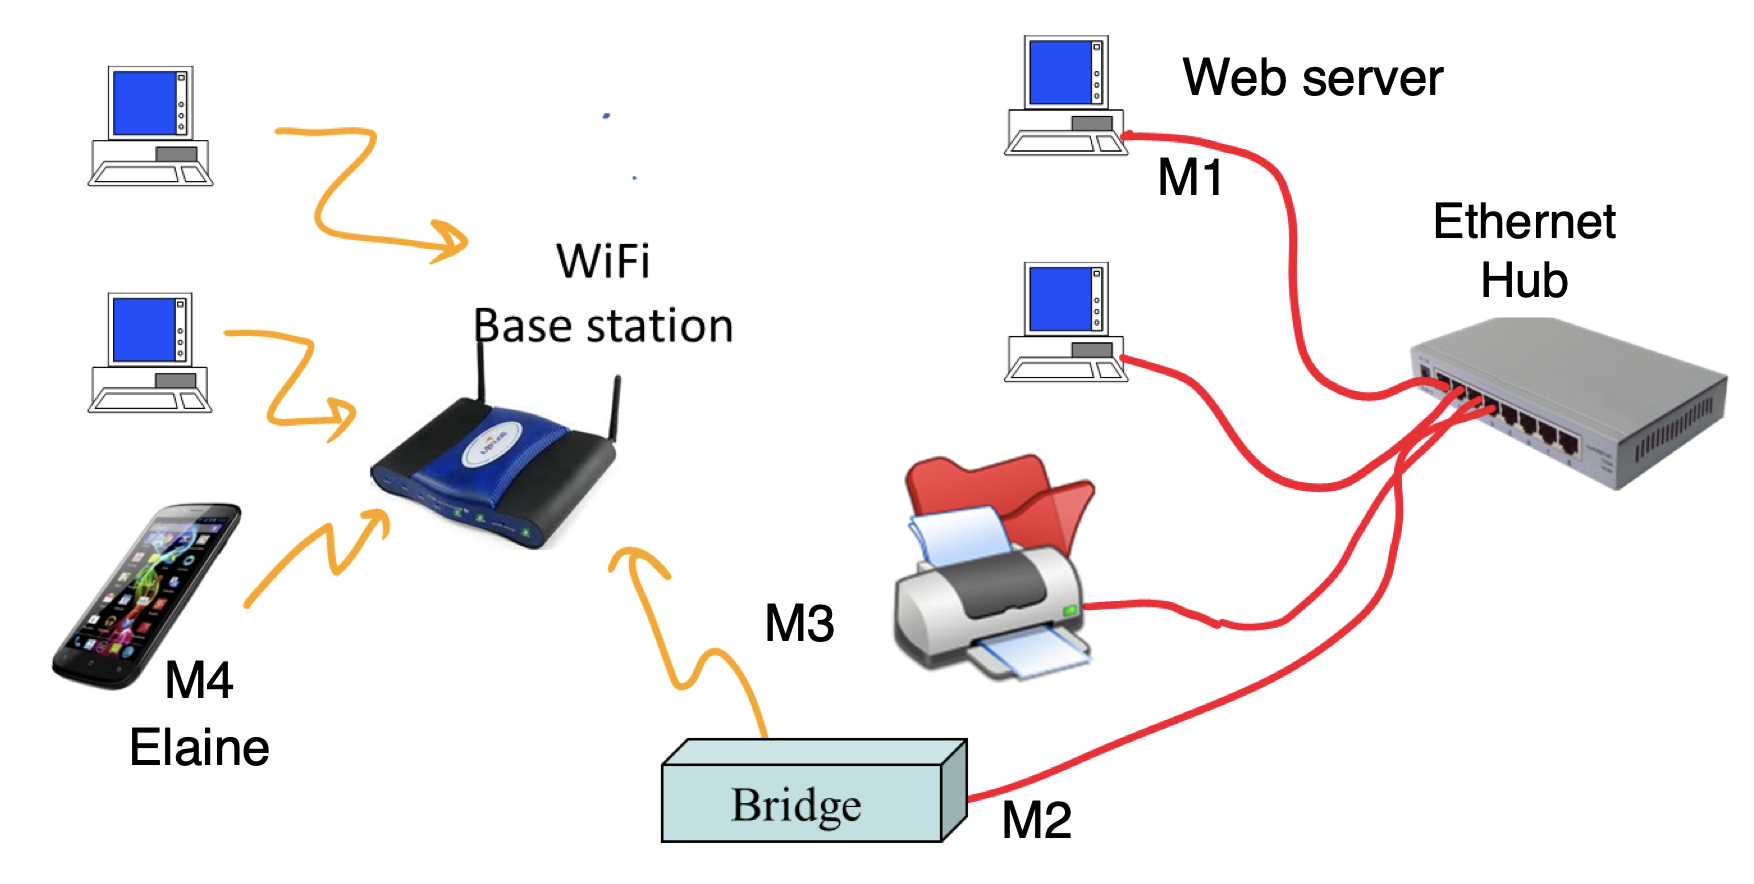
\includegraphics[width=0.8\textwidth]{images/bridge}
    \label{fig:LABEL}
\end{figure}

\newpage
\section*{WiFi Access Point (a typical bridge)}

\begin{itemize}
	\item Combines:
		\begin{itemize}
			\item a WiFi base station (implements the WiFi MAC protocol)
			\item a switch with an Ethernet backend (called the \textcolor{red}{Distribution System})
		\end{itemize}
	\item WiFi frames differ from Ethernet frames; they include \textit{\textcolor{blue}{3 MAC addresses}} source, dest and access-point
\end{itemize}

% Quick centered image
\begin{figure}[H]
    \centering
    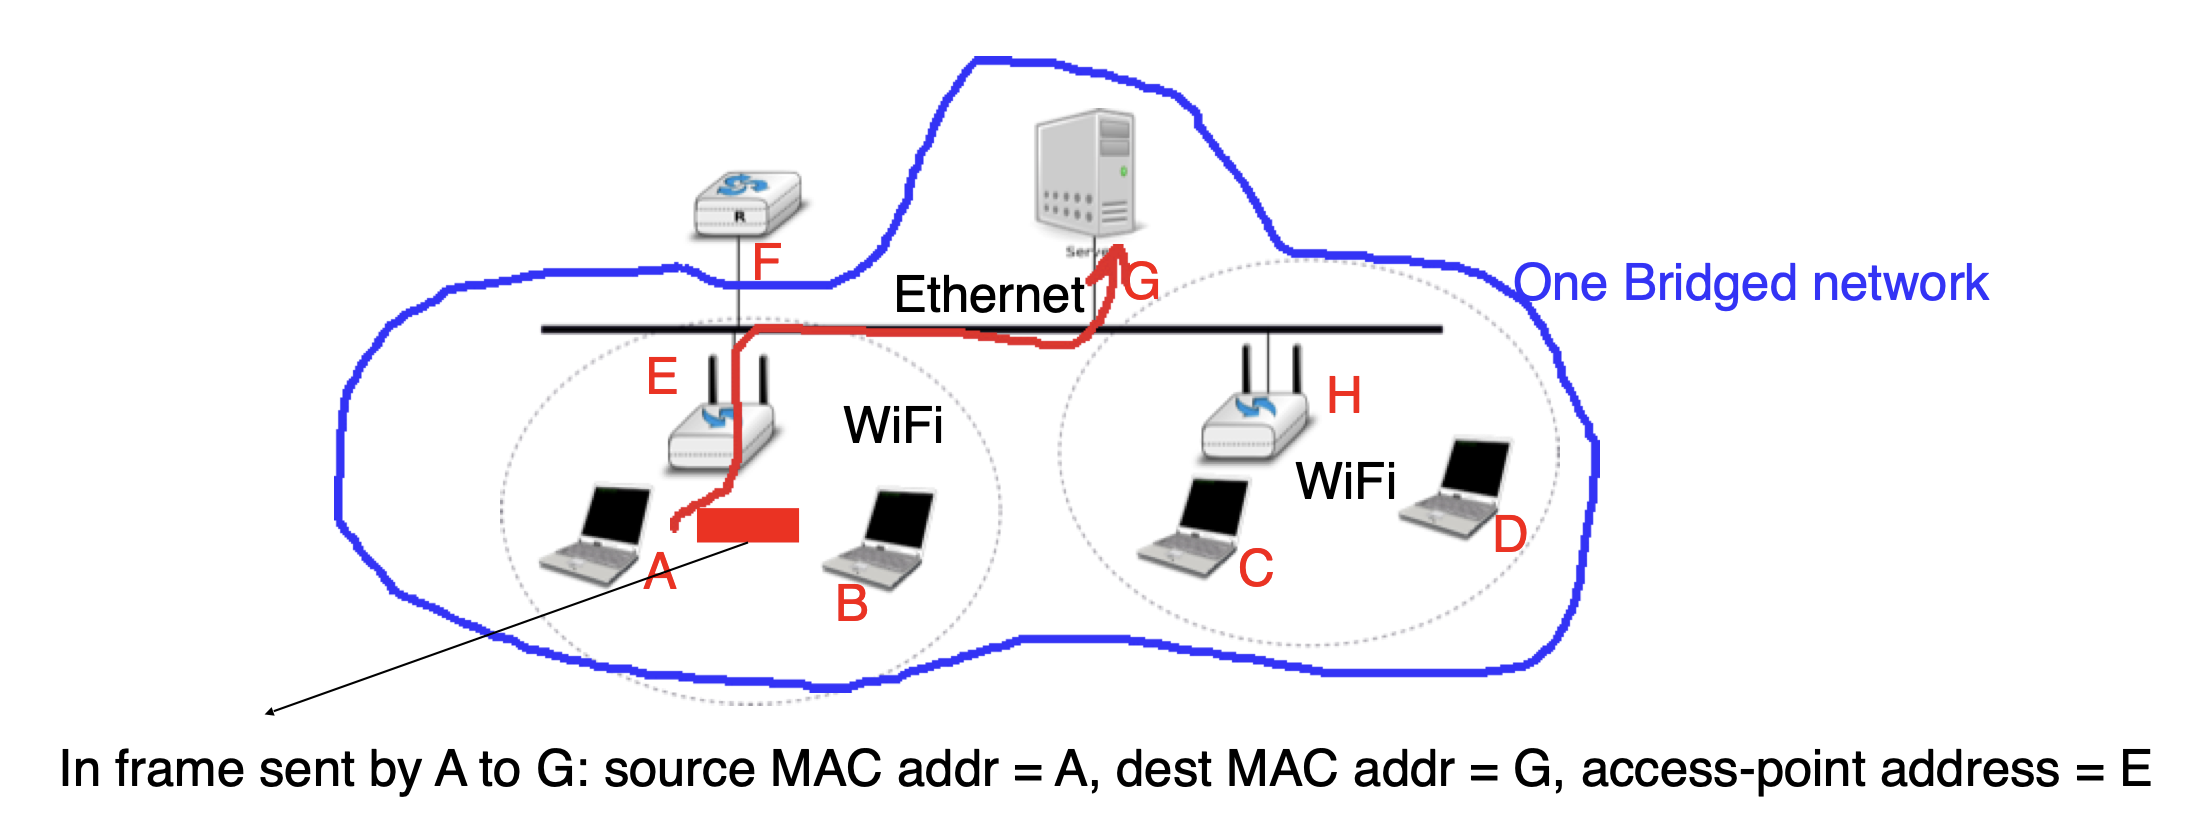
\includegraphics[width=1\textwidth]{images/wifi}
    \label{fig:LABEL}
\end{figure}

\section*{WiFi Access Point with Wireless Distribution System}

\begin{itemize}
	\item WiFi backend instead of Ethernet:
		\begin{itemize}
			\item WiFi base stations are interconnected via WiFi relays, which act as switches
		\end{itemize}
	\item WiFi frames include $\leq$ \textcolor{blue}{\textit{MAC addresses}} source, dest, transmitter/receiver delays
\end{itemize}

% Quick centered image
\begin{figure}[H]
    \centering
    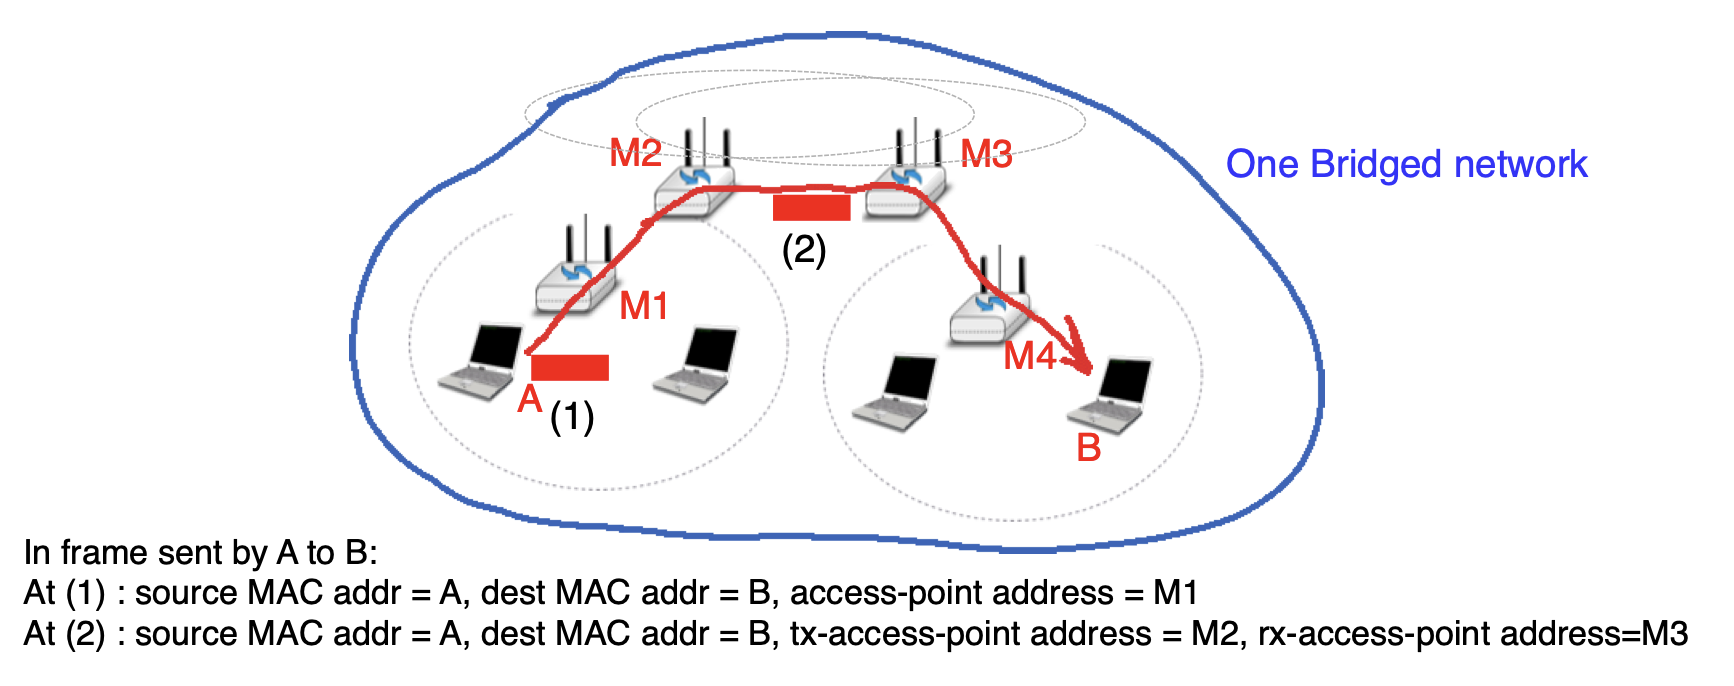
\includegraphics[width=1\textwidth]{images/wifi-wireless}
    \label{fig:LABEL}
\end{figure}

\begin{minipage}{0.5\textwidth}
\begin{tcolorbox}[
  colback=gray!15,     % background color
  colframe=black!50,    % border color
  boxrule=1pt,       % border thickness
  arc=3mm,             % rounded corners
  left=4mm, right=4mm, top=2mm, bottom=2mm % padding
]
\textbf{Web server send one IP packet to Elaine. At (1), the MAC destination address is...}
% Quick centered image
\begin{figure}[H]
    \centering
    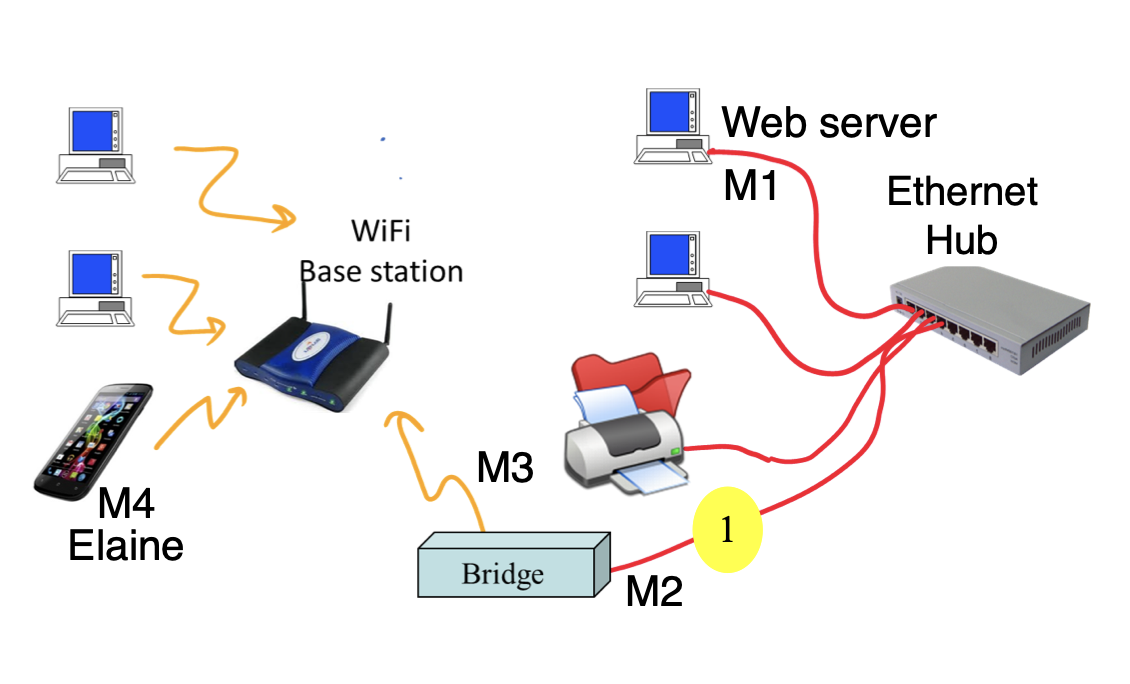
\includegraphics[width=1\textwidth]{images/elaine-1}
    \label{fig:LABEL}
\end{figure}
\vspace{0.3cm}
A. M1 \\
B. M2 \\ 
C. M3 \\
D. M4 \\
E. I don't know \\

\textbf{Answer}: M4
\end{tcolorbox}
\end{minipage}
\hfill
\begin{minipage}{0.5\textwidth}
\begin{tcolorbox}[
  colback=gray!15,     % background color
  colframe=black!50,    % border color
  boxrule=1pt,       % border thickness
  arc=3mm,             % rounded corners
  left=4mm, right=4mm, top=2mm, bottom=2mm % padding
]
\textbf{Web server sends one IP packet to Elaine. At (1), the MAC destination address is...}
% Quick centered image
\begin{figure}[H]
    \centering
    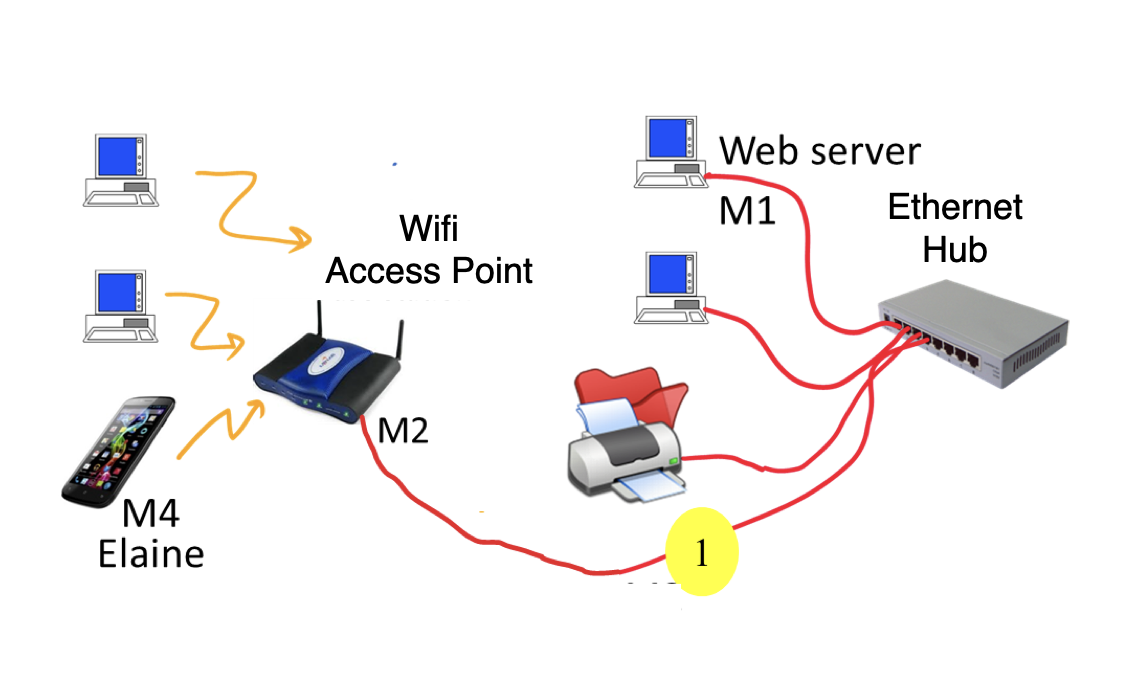
\includegraphics[width=1\textwidth]{images/elaine-2}
    \label{fig:LABEL}
\end{figure}
\vspace{0.3cm}
A. M1 \\
B. M2 \\
C. M4 \\
D. I don't know \\

\textbf{Answer}: M4
\end{tcolorbox}
\end{minipage}

\textcolor{blue}{Which topology is more efficient? Which one uses resources better?}

\textbf{Answer:} the one without the bridge. 

In the first case, the WiFi base station is not connected to a wired infrastructure and it acts as a Wifi \textcolor{blue}{\textit{range extender}}. Instead, it is connected wirelessly to a bridge. This is not very efficient because all WiFi traffic that goes to the bridge uses WiFi twice, once to access the base station, once to go from base station to the bridge. 

The second case is the typical use of an \textcolor{red}{\textit{access point}}. The base station contains a bridge and is itself connected by Ethernet to the rest of the network.
\end{document}

